\section{实验结果与对比}
并排图片显示:\\
 \begin{figure}[hbtp]
\begin{minipage}[t]{0.5\linewidth}
\begin{tikzpicture}[scale=0.5]
  \tkzInit[xmin=-4,xmax=9,ymin=-3,ymax=9]
  \tkzClip
  \tkzDefPoint(2,3){A}
  \tkzDefPoint[shift={(2,3)}](31:8){B}
  \tkzDefPoint[shift={(2,3)}](158:8){C}
  \tkzDrawSegments[color=red,line width=1pt](A,B A,C)
  \tkzProtractor[scale=1.25,with=full,return](A,C)
\end{tikzpicture}
\caption{图片1}
\end{minipage}
\hfill
\begin{minipage}[t]{0.5\linewidth}
\centering
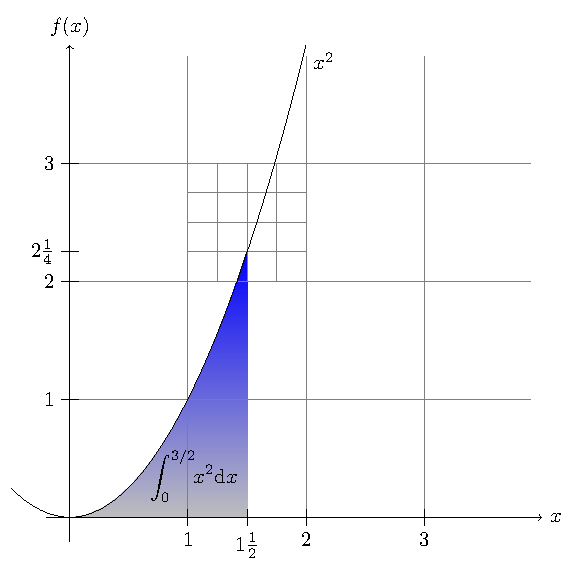
\includegraphics[width=2in]{parabola-plot.pdf}
%\centering
\caption{图片2}
\end{minipage}

\end{figure}